%!TEX root = root.tex

\chapter{20/20+: a machine learning method to predict cancer driver genes}
\label{chap:ch3}
\chaptermark{20/20+}

\section{Introduction}

The first exomic analyses attempted to identify candidate driver genes as those having more mutations than expected from some presumed background somatic mutation rate, corrected for base context, gene size, and other variables \cite{RN78, RN4}. Subsequent work has considerably refined the variables involved in determining whether a gene is more mutated in cancers than expected by chance. This has led to a variety of \q{significantly mutated gene} methods that adjust for covariates such as replication timing and gene expression as well as including more sophisticated metrics of mutational base contexts \cite{RN13, RN43}. Although methods have been extended to utilize gene expression \cite{RN80, RN84, RN81, RN83, RN79, RN82}, I will focus solely on driver gene analysis based on somatic point mutations.

An alternative method to finding cancer drivers employs a ratiometric approach. Rather than attempting to determine whether the observed mutation rate of a gene in cancers is higher than expected by chance, these methods simply assess the composition of mutations normalized by the total mutations in a gene. The ratiometric 20/20 rule \cite{RN25} evaluates the proportion of inactivating mutation and recurrent missense mutations in a gene of interest. Other ratiometric approaches use mutation functional impact bias \cite{RN86, RN53}, mutational clustering patterns \cite{RN87, RN54, RN71}, or patterns of mutation composition \cite{RN71}. Here, I describe a machine-learning-based, ratiometric method (20/20+) that formalizes and extends the original 20/20 rule and enables automated integration of multiple features of positive selection.

\section{Original 20/20 rule}

The original 20/20 rule was a manually designed set of decision rules to identify cancer driver genes as either an oncogene or tumor suppressor gene (\autoref{fig:2020rule}) \cite{RN25}. The name derives from the rule that oncogenes should have at least 20\% of mutations being recurrent (observed more than once) and tumor suppressor genes should have at least 20\% inactivating mutations (i.e., frame shift indels, nonsense mutations, etc.). In addition, there are count thresholds that are specifically tuned for analyzing a specific version of the COSMIC database \cite{RN95}. When I applied this rule to a later version of COSMIC, it had inadequate specificity (data not shown). Moreover, scaling the count thresholds relative to database size also produced similar results, suggesting additional manual curation of results would be necessary. Consistent with this observation, the 20/20 rule had good performance at distinguishing oncogenes versus tumor suppressor genes within already pre-defined driver genes \cite{RN88}.

\begin{figure}
  \centering
  \makeatletter
  \let\@currsize\normalsize
  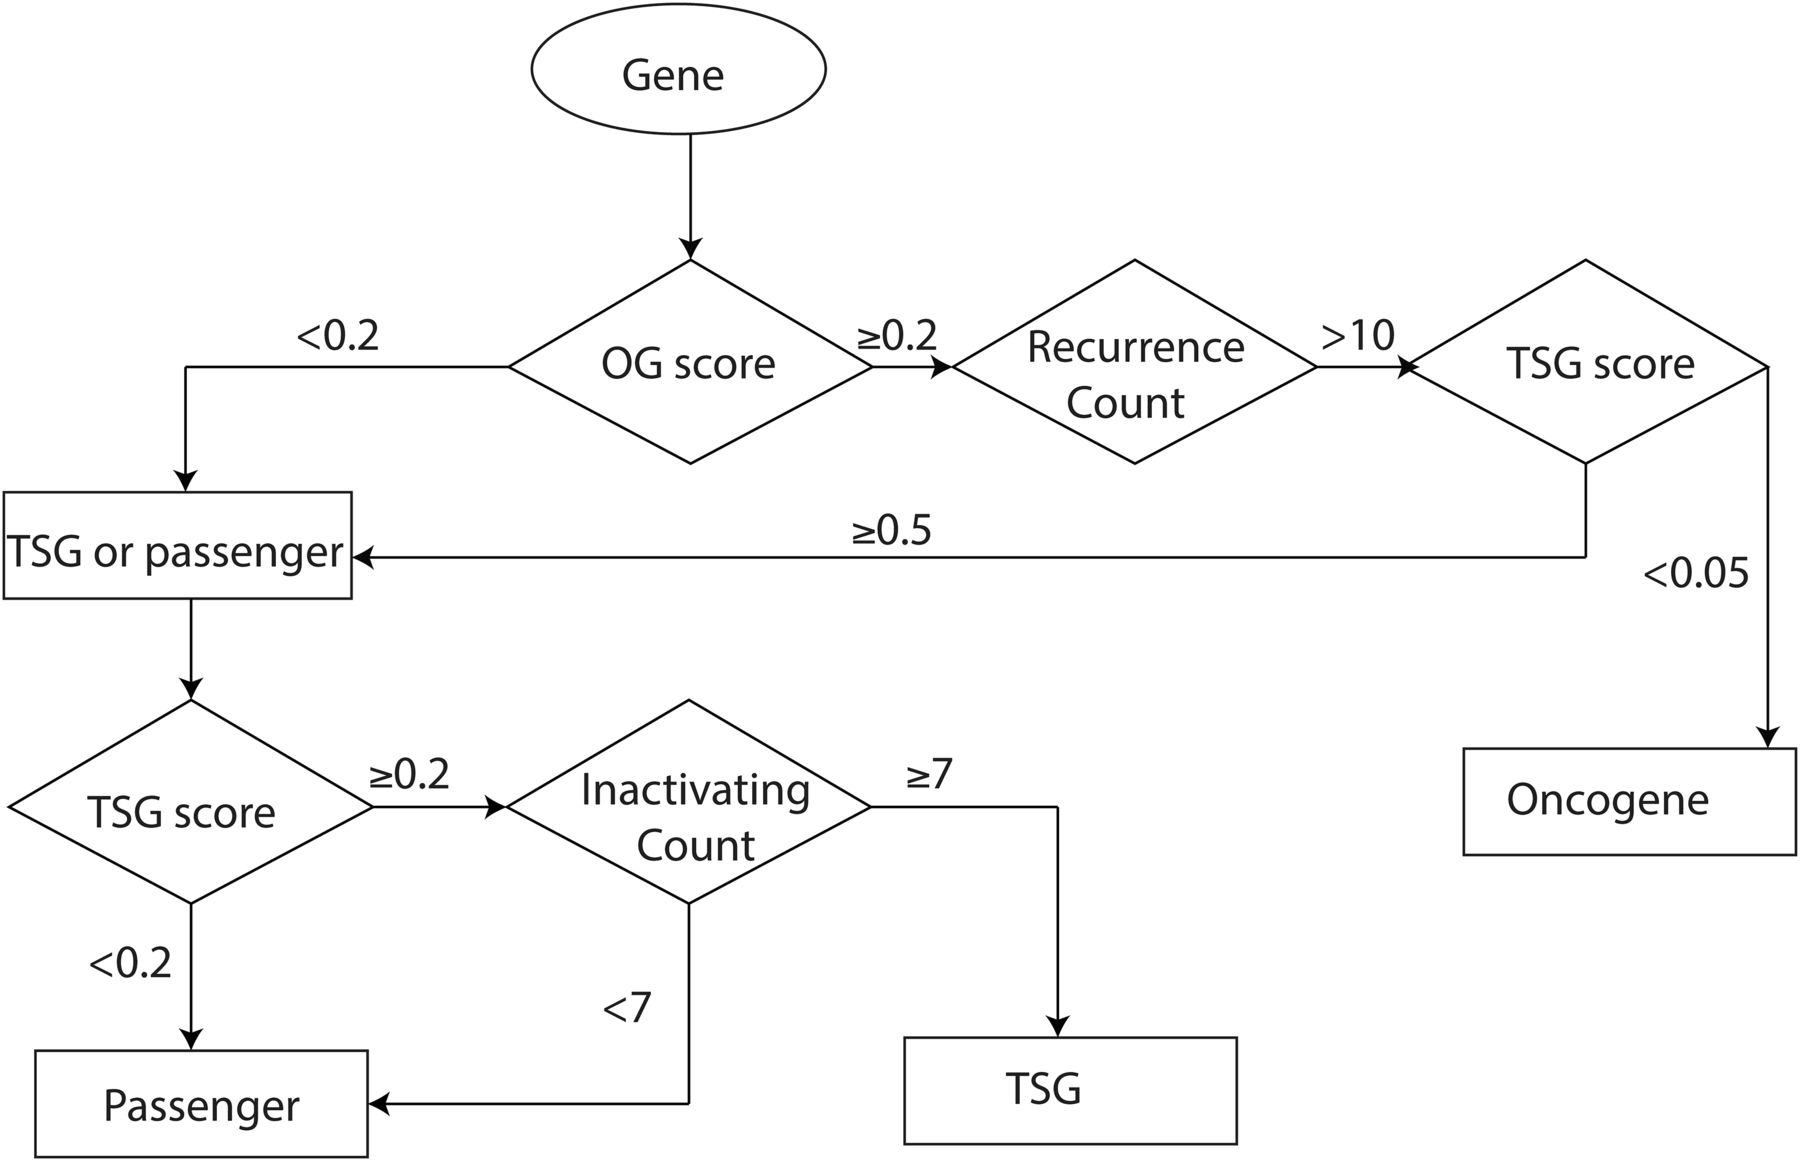
\includegraphics[width=0.9\linewidth]{figures/chapter3/2020_rule.jpg}
  \caption[Decision tree underlying 20/20 rule.]{Decision tree underlying 20/20 rule. Each gene is input into the tree and oncogene (OG) and tumor suppressor gene (TSG) score computed. Thresholds of each score and the numerator of the OG score (recurrence count) and TSG score (inactivating count) are used to determine whether a gene is an OG, TSG, or passenger.}
  \label{fig:2020rule}
\end{figure}

\section{Machine learning prediction of cancer driver genes}

Using machine learning, 20/20+ trains a random forest to leverage many features simultaneously to predict cancer driver genes. Random forests outperformed logistic regression, boosting, and support vector machines (data not shown). I will first go over the mathematical background of random forests and then describe the implementation in 20/20+.

\subsection{Mathematical overview of random forests}

\subsubsection{Decision tree}

Since my focus will be on classification, a decision tree $\pi(X)$ will return 1 if the prediction is a cancer driver and 0 for a passenger. A decision tree is constructed from a set of possible questions $Q=\{Q_1,\ldots,Q_N\}$, with a question taking the following form,

\begin{equation}
Q_.(X)=I_{X_i \leq c}
\end{equation}

where $I$ is the indicator function, $X_i$ is the i'th feature value, and $c$ is a constant. The question asked by a decision tree depends on the previous question asked. To keep track of order of questions, the index of the first question will be denoted $\rho_1$, where $\rho_1\in\{1\ldots N\}$. The second question will therefore be a function of the answer from the first question, $\rho_2=\rho_2(a_1)$, where $a_1=Q_{\rho_1}$. More generally there is a series of questions $\beta_n=\{Q_{\rho_1}=a_1,\ldots,Q_{\rho_{n-1}}=a_{n-1}\}$ prior to the n'th question.

Each question will split training examples depending on the answer to the question. The goal of the decision tree is to utilize questions that reduce the uncertainty in the distribution of class labels. I will regard the distribution of class labels as the probability of observing a class label given the answer to a question n as follows,

\begin{equation}
p_k=Pr⁡(Y=1|Q_{ρ_n}=k,\beta_n)
\end{equation}

where $k$ is the answer to the question and $p_k$ is the proportion of labeled drivers. For the decision tree algorithm, the best question defined by the gini impurity is used at each step:

\begin{equation}
\rho_n=\argmin_{1 \leq b \leq N}{2\sum_{k=0}^{1}{Pr[Q_b=k]p_k(1-p_k)}}
\end{equation}

There are various practical criteria to decide when to stop asking further questions in a decision tree, but I will not cover this here. Assuming a decision tree is constructed, the predicted class is chosen by the most likely class following the terminal question.

\begin{equation}
\pi(X) = \argmax_l{Pr(Y=l|\beta_*)}
\end{equation}

where $l\in \{0,1\}$ is the class label and $\beta_*$ contains the history of answers for all questions. 

\subsubsection{Random Forest}

A random forest is an ensemble of many randomized decision trees \cite{RN41, RN40}, where each tree is trained on a random selection of training set examples and candidate features, via a recursive splitting process \cite{RN89}. This involves constructing each tree $\pi_j$ from a bootstrapped sample of the training data $D_j=\{(X(i),Y(i)),\ldots\}_{i=1..m}$. Then instead of allowing all questions for each split, a random subset of questions is used $Q^s\subset Q$, were the number of features $s$ is usually taken to be proportional to the square root of the total features p,  $|s|=\sqrt{p}$. Lastly, once $J$ decision trees are constructed, random forest predictions result in a score between 0 and 1 that reflects the proportion of trees agreeing with the class label of cancer driver:

\begin{equation}
f(X) = \frac{1}{J}\sum_{j=1}^J{\pi_j(X)}
\end{equation}

\subsection{Random Forest implementation}

Although the above mathematical description of a random forest was in terms of two classes (drivers and passengers) for simplicity, random forest classification also extends to multi-class classification. 20/20+ uses a three-class classifier which predicts a gene as either an oncogene, tumor suppressor genes, or passenger gene. I used the set of oncogenes and tumor suppressor genes identified by the original 20/20 rule as a training set \cite{RN25}. Considering cancer driver genes (oncogenes or tumor suppressor genes) constitute only a small proportion of all genes, I labeled all other genes as passenger for the purpose of training. 

\subsubsection{Features}

I designed a set of 24 predictive features and whose feature importance is shown in \autoref{fig:2020features}, as assessed by the mean decrease in gini impurity. Many of the features are components of the 20/20 rule OG and TSG scores, and I included several ratiometric features not in the original 20/20 rule, for example, ratio of missense to silent mutations, as well as features that represented mutation functional impact and gene importance. Normalized missense entropy, a measure of positional clustering, was calculated as follows:

\begin{equation}
E_k = \frac{\sum_i{p_i\log_2{p_i}}}{\log_2{k}}
\end{equation}

where $k$ is the total number of missense mutations in a gene and $p_i$ = (count of missense mutations in the I'th codon)/k. Three of the 24 features represented p-values and were calculated using the monte carlo simulation described in \autoref{sec:monte_carlo}.

\begin{figure}
  \centering
  \makeatletter
  \let\@currsize\normalsize
  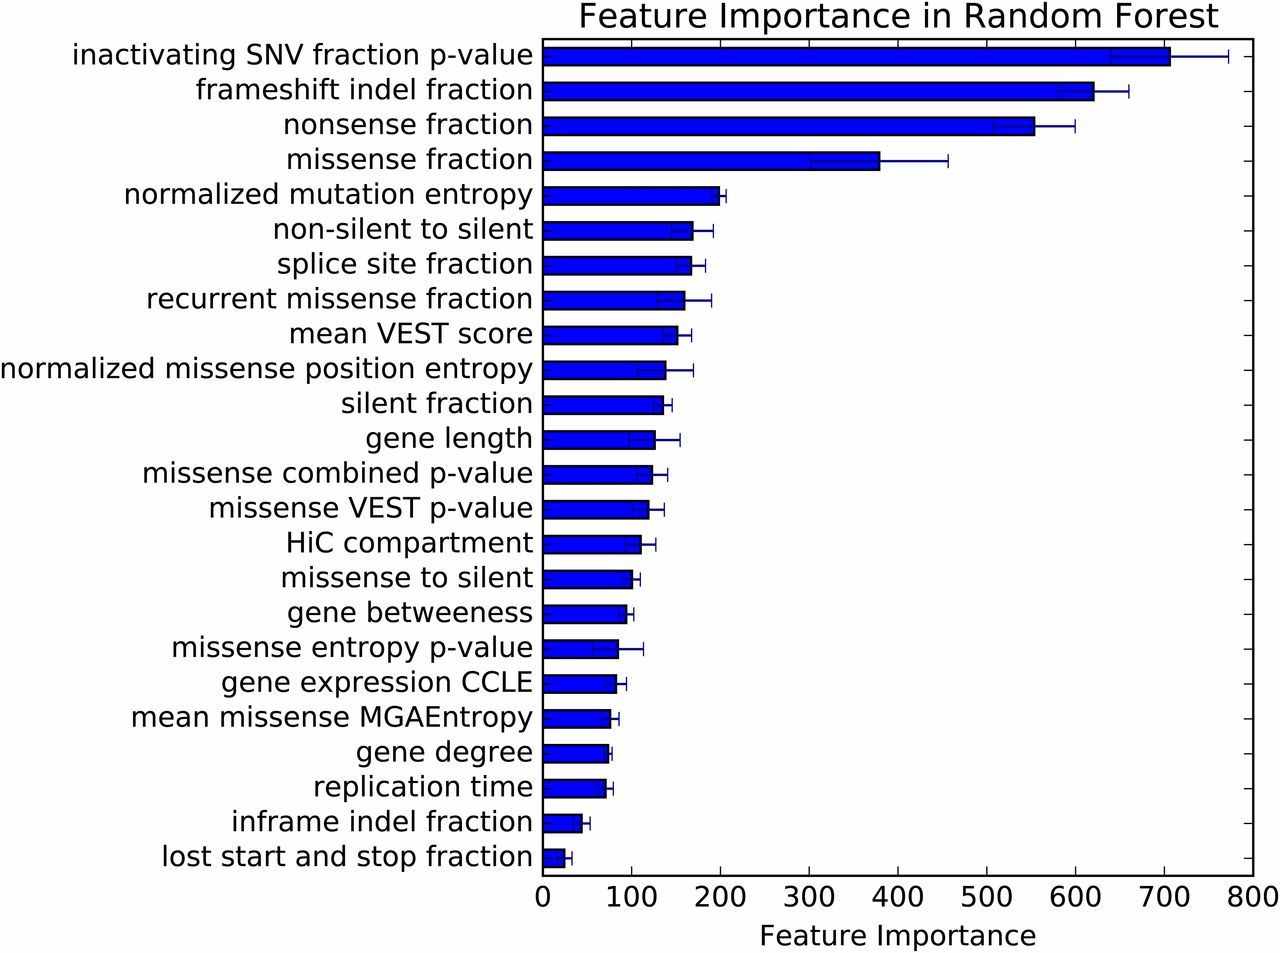
\includegraphics[width=0.9\linewidth]{figures/chapter3/feature_importance.jpg}
  \caption[Random Forest feature importance ranking for the 24 predictive features.]{Random Forest feature importance ranking for the 24 predictive features. The mean decrease in Gini index is plotted for each feature. Error bars indicate SD when feature importance calculation was repeated on 10 different cross-validation partitions. CCLE, Cancer Cell Line Encyclopedia \cite{RN13}; HiC, 3D chromatin interaction capture \cite{RN13}; MGAEntropy, Shannon entropy in column of a vertebrate genome 46-way alignment corresponding to location of the mutation \cite{RN90}; SNV, single-nucleotide variant; VEST, Variant Effect Scoring Tool \cite{RN30}.}
  \label{fig:2020features}
\end{figure}

\subsubsection{Handling class imbalance}

With only 54 OGs and 71 TSGs labeled by the original 20/20 rule, the number of passenger genes far exceeds the number of labeled driver genes, creating a problematic class imbalance \cite{RN93}. I use a subsampling approach, previously recommended for random forests \cite{RN92}, in which for my case the passenger genes are sampled at a 1:1 ratio to OGs plus TSGs. To compensate for the remaining OG and TSG imbalance, the Random Forest is trained with class weights inversely proportional to the sampled frequency of the class. Predictions were made with a random forest of 200 trees. The number of trees only had minor impact on the overall performance. I used 10-fold gene hold-out cross-validation to avoid overfitting. The procedure of 10-fold cross-validation was repeated five times (1,000 trees in total), and the resulting scores from each gene were aggregated to limit minor fluctuations in scores due to randomization in the cross-validation folds.

\subsubsection{Random forest prediction}

Each gene was scored as the fraction of trees that voted for oncogene, tumor suppressor gene, or passenger gene. A driver score for each was calculated as the sum of the oncogene and tumor suppressor gene scores. A driver score was included in case the gene was likely a cancer driver, but the precise type of cancer driver gene was hard to determine.

\section{Statistical significance}

The statistical significance of each gene score was computed with an extension of the Monte Carlo simulation algorithm described in \autoref{sec:monte_carlo}. For each gene, the Monte Carlo simulation was repeated 10 times, and for each simulation all 24 features were computed. In this process, protein interaction network features (degree and betweenness) were, additionally, permuted as a pair. The features of gene length, replication timing, HiC value, and average Cancer Cell Line Encyclopedia (CCLE) gene expression were not altered. Next, each \q{simulated} gene was scored with the Random Forest previously trained on the real data. The resulting OG, TSG, and driver scores for all simulated genes were used as an empirical null distribution. To compute a P value for a gene score, I used the fraction of simulated genes with a score equal to or greater than the score. P values were adjusted by the Benjamini-Hochberg method \cite{RN94} for multiple hypotheses. I compute a Benjamini-Hochberg q-value as follows,

\begin{equation}
q(i) = \min{\left(\min_{i..n}{\frac{p(i)}{i/n}}, 1 \right)}
\end{equation}

where $p(i)$ is the i'th smallest p-value, $q(i)$ is the corresponding q-value, n is the total number of p-values, and $\min_{i..n}$ is the cumulative minimum from index n to i. Consistent with other driver gene prediction methods, I considered a gene to be significant ($q \leq 0.1$) if any of the OG, TSG, or driver scores were significant. The strategy of converting p-values to q-values is for convenience and does not change the significant p-values by the procedure originally outlined by Benjamini and Hochberg \cite{RN94}.

\section{Conclusions}

In this chapter, I developed a new method, 20/20+, which addresses two major issues with the original 20/20 rule: use of a limited number of features and a lack of a statistically principled threshold to limit false positives. 20/20+ uses the random forest algorithm to make predictions using a non-linear combination of features. Importantly, 20/20+ uses ratiometric features to normalize artefactual differences between cancer types and regions of the genome. Because Random Forests do not intrinsically include hypothesis testing techniques, I used simulated mutations to assess the statistical significance of scores. P-values were estimated from a simulated null distribution, controlling for sequence composition, and corrected for multiple testing with the Benjamini-Hochberg method \cite{RN94}. The application and benchmarking of 20/20+ will be considered in Chapters 4 and 7.

